\documentclass[tikz,border=4pt]{standalone}

\usepackage{amsmath}
\usepackage{amssymb}
\usetikzlibrary{arrows.meta,calc}

\definecolor{viablue}{HTML}{6CA2C6}
\definecolor{axisgray}{HTML}{555555}
\definecolor{guidegray}{HTML}{999999}

\begin{document}
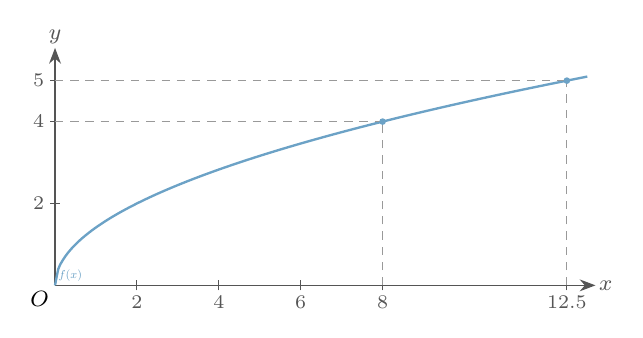
\begin{tikzpicture}[
    scale=0.52,
    >=Stealth,
    axis/.style={->, semithick, axisgray},
    guide/.style={dash pattern=on 3pt off 2.5pt, guidegray},
    curve/.style={line width=0.85pt, viablue},
    tick/.style={axisgray, thin},
    lbl/.style={font=\footnotesize, inner sep=1pt},
    numlbl/.style={font=\scriptsize, inner sep=0.5pt},
    point/.style={fill=viablue, circle, inner sep=0pt, minimum size=2.4pt}
  ]
  % Axes
  \draw[axis] (0,0) -- (13.2,0) node[right, lbl] {$x$};
  \draw[axis] (0,0) -- (0,5.8) node[above, lbl] {$y$};
  \node[lbl, below left=1pt] at (0,0) {$O$};

  % Axis ticks and labels
  \foreach \x in {2, 4, 6, 8} {
    \draw[tick] (\x,-0.12) -- (\x,0.12) node[below=5pt, numlbl] {$\x$};
  }
  \draw[tick] (12.5,-0.12) -- (12.5,0.12) node[below=5pt, numlbl] {$12.5$};
  \foreach \y in {2, 4} {
    \draw[tick] (-0.12,\y) -- (0.12,\y) node[left=5pt, numlbl] {$\y$};
  }
  \draw[tick] (-0.12,5) -- (0.12,5) node[left=5pt, numlbl] {$5$};

  % Function graph
  \draw[curve, domain=0:13, samples=160, smooth]
    plot (\x, {sqrt(2*\x)})
    node[pos=0.82, above right=1pt, lbl, text=viablue] {$f(x)$};

  % Read f(8) = 4
  \draw[guide] (8,0) -- (8,4);
  \draw[guide] (0,4) -- (8,4);
  \node[point] at (8,4) {};

  % Read input when f(x) = 5
  \draw[guide] (0,5) -- (12.5,5);
  \draw[guide] (12.5,0) -- (12.5,5);
  \node[point] at (12.5,5) {};
\end{tikzpicture}
\end{document}
